
% License:
% CC BY-NC-SA 3.0 (http://creativecommons.org/licenses/by-nc-sa/3.0/)
%
%%%%%%%%%%%%%%%%%%%%%%%%%%%%%%%%%%%%%%%%%

%----------------------------------------------------------------------------------------
%	PACKAGES AND OTHER DOCUMENT CONFIGURATIONS
%----------------------------------------------------------------------------------------

\documentclass[paper=a4, fontsize=11pt]{hitec} % A4 paper and 11pt font size

\usepackage[T1]{fontenc} % Use 8-bit encoding that has 256 glyphs
\usepackage[english]{babel} % English language/hyphenation
\usepackage{amsmath,amsfonts,amsthm} % Math packages

\usepackage{caption}
\usepackage{subcaption}
\usepackage{graphicx}

\usepackage{float}

\usepackage{blindtext} %for enumarations

\usepackage[]{hyperref}  %link collor

%talbe layout to the right
%\usepackage[labelfont=bf]{caption}
%\captionsetup[table]{labelsep=space,justification=raggedright,singlelinecheck=off}
%\captionsetup[figure]{labelsep=quad}

%\usepackage{sectsty} % Allows customizing section commands
%\allsectionsfont{\centering \normalfont\scshape} % Make all sections centered, the default font and small caps

\usepackage{fancyhdr} % Custom headers and footers
\pagestyle{fancyplain} % Makes all pages in the document conform to the custom headers and footers
\fancyhead{} % No page header - if you want one, create it in the same way as the footers below
\fancyfoot[L]{} % Empty left footer
\fancyfoot[C]{} % Empty center footer
\fancyfoot[R]{\thepage} % Page numbering for right footer
\renewcommand{\headrulewidth}{0pt} % Remove header underlines
\renewcommand{\footrulewidth}{0pt} % Remove footer underlines
\setlength{\headheight}{13.6pt} % Customize the height of the header

\numberwithin{equation}{section} % Number equations within sections (i.e. 1.1, 1.2, 2.1, 2.2 instead of 1, 2, 3, 4)
\numberwithin{figure}{section} % Number figures within sections (i.e. 1.1, 1.2, 2.1, 2.2 instead of 1, 2, 3, 4)
\numberwithin{table}{section} % Number tables within sections (i.e. 1.1, 1.2, 2.1, 2.2 instead of 1, 2, 3, 4)

%\setlength\parindent{0pt} % Removes all indentation from paragraphs - comment this line for an assignment with lots of text


\setlength\parskip{4pt}

%----------------------------------------------------------------------------------------
%	TITLE SECTION
%----------------------------------------------------------------------------------------

\newcommand{\horrule}[1]{\rule{\linewidth}{#1}} % Create horizontal rule command with 1 argument of height

\title{	
\normalfont \normalsize 
\textsc{The Hong Kong Polytechnic University\\ SingularityNet} \\ [25pt] % Your university, school and/or department name(s)
\horrule{0.5pt} \\[0.4cm] % Thin top horizontal rule
\huge  Causal analysis in Networks via Deep Neural-Symbolic Learning: a preliminary result \\ % The assignment title
\horrule{2pt} \\[0.5cm] % Thick bottom horizontal rule
}

\author{  Andres Suarez-Madrigal, Tesfa Yohannes, Ben Goertzel} % Your name

\date{\normalsize\today} % Today's date or a custom date

\begin{document}
%\nocite{*}
\maketitle % Print the title

% \newpage
\begin{abstract}

%{\noindent{\Large Abstract} }\\

This report presents preliminary results on the processing of telemetry data, as part of a pipeline that attempts to find the cause of anomalies in the network that produces the data.
The scope of the whole project is summarized in the Introduction, in order to offer the appropriate context to this report, but the focus of the latter is on the visualization efforts showing that one of the main assumptions made in our pipeline is justified: that it is possible to represent the network data in a way that distinguishes normal operation from anomalous states.\\
%\textbf{Key words:} some keywords 
    
\end{abstract}

%\newpage
% \tableofcontents

%----------------------------------------------------------------------------------------
%	Section 1
%----------------------------------------------------------------------------------------




%how to cite
%\cite{Seow2011}

%how to add figure
% \begin{figure}[h!]
% 	\centering
% 	\includegraphics[width=0.8\linewidth]{Figure/Total-consumption.jpg}
% 	\caption{Total Consumption by End-Use Sector, 1949-2011 \cite{Apostolos2013}}
% 	\label{fig:TotalConsumption}
% \end{figure}



\newpage
\section{Introduction}

The current project explores a method to predict anomalous events in the dynamics of a network, via finding their causes.
The main idea in the method is to find the grammar of the network -- its implicit dynamical structure-- in an unsupervised manner, starting from telemetry data of its different components.
If such a grammar can be obtained, then it would be possible to predict (with a certain confidence) an anomaly when observing dynamics that preceed such a state in the grammar.
This would be similar to a situation in language processing where, after observing a sequence of words that form a sentence's subject (e.g. determiner-adjective-noun), we can expect a verb to follow.\\

This project will leverage SingularityNet's Unsupervised Language Learning (ULL) pipeline, which attempts to find the grammar implicit in a given corpus of sentences.
In order to process the network data with such pipeline, the process can be divided into three stages:
\begin{enumerate}
\item Abstract the network dynamics by converting the state of the network at each timestep into a real-valued vector (or a set of vectors).
\item Using symbolic dynamics techniques, convert the dynamics of the network embedding vector(s) into a sequence of symbols; these sequences would be functionally equivalent to a natural language corpus in the ULL project.
\item Apply a suitable version of the ULL pipeline to the sequences obtained in step 2 (the sentences), in order to learn the network grammar.
\end{enumerate}

The first step could be done in a number of ways.
One popular and successful way to create distributed representations is using Neural Networks.
Deep Neural Networks like graph2seq have been used to abstract graphs, with some success 
\cite{venkatakrishnan_graph2seq_2018}.\\
TESFA, YOU CAN ADD SOME STUFF HERE.

Another approach for creating embeddings is to use the features as they come from the telemetry data.
We follow a similar processing as done by \cite{putina_telemetry-based_2018}.

For step 3, we need to adapt the ULL pipeline to our purposes: instead of having a natural language sentence where every word is presented to the algorithm at the same time, we would be dealing with a continous stream of tokens representing the state of the network at different times.
In particular, the parser used in the ULL pipeline needs to be replaced by one that handles a continous stream of tokens.
For this purpose, we implemented a continuous version of the MST-parser proposed by Yuret \cite{Yuret1999}\footnote{Code available at https://github.com/glicerico/stream-parser}


%----------------------------------------------------------------------------------------
%	Section 2
%----------------------------------------------------------------------------------------

\newpage
\section{Embeddings}
\label{sec:embeddings}

A crucial part of the proposed pipeline is to represent the obtained raw telemetry data in a way that abstracts the state of the network, distiniguishing clearly when it is in an anomalous state.
Deep neural networks have been used for non-dynamical graphs \cite{venkatakrishnan_graph2seq_2018}, where the structure of the graph is converted to a continous vector for each timestep.
We need a DNN that can also process the dynamical behaviour of our data into the graph.

Another possibility is to use the telemetry data directly, in a fashion similar to Putina et al.\cite{putina_telemetry-based_2018} to feed their clustering algorithm.
However, what is important in our case is that the representations used can distinguished between normal and anomalous network operation.
In order to explore this, we decided to visualize the data and find out if some of the given features could be projected into a lower dimensional space, where a distinction between anomalous and normal behavior is clear.

We started with the data available in the \textbf{telemetry} repository\footnote{https://github.com/cisco-ie/telemetry}, which contains data from experiments with different failure conditions.
The databases contain readings for a subset of the available features for all nodes at different timesteps, pertaining to different Yang paths.
We first constructed a network embedding for each unique timestep, independent of its origin node or Yang path.
Using the ground truth information provided with the datasets, we also tag each timestep as 'anomaly' or 'normal', to use during visualization.
Given the high dimensionality of the resulting vectors, we use the online \textit{Embedding Projector} feature of TensorFlow\footnote{Available at https://projector.tensorflow.org/} to project and visualize them.
Figure \ref{fig:dataset3_all_P100} shows the t-SNE projection from dataset \#3, with blue points representing 'normal' behavior, and red ones timesteps where an 'anomaly' is present.
We notice that this projection does not show a clear division between the two states of interest from this embeddings everywhere.
Instead, it seems that the data can be grouped by the Yang path that produced it, as can be seen in figure \ref{fig:dataset3_all_P100_names}.

\begin{figure}[h!]
	\centering
	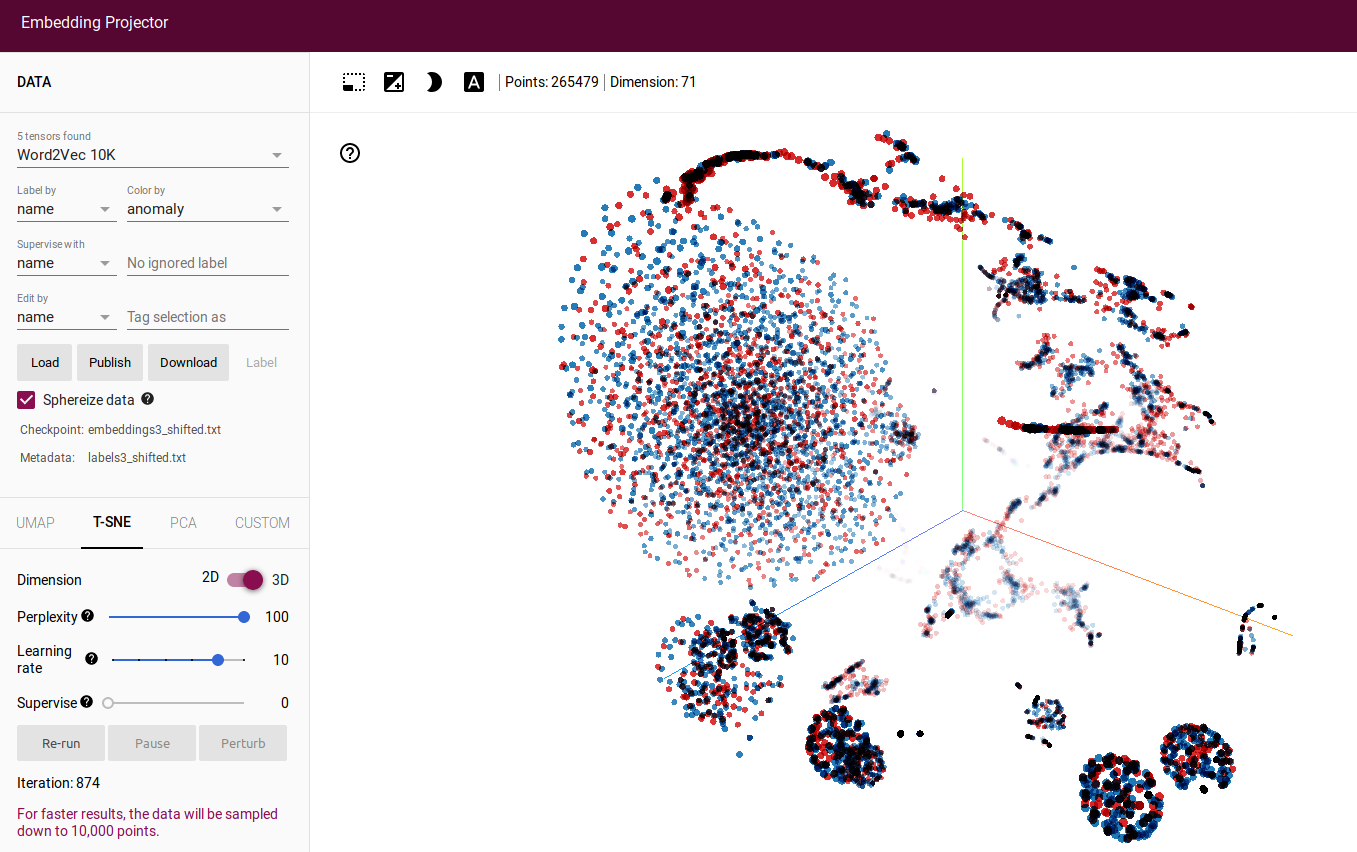
\includegraphics[width=0.8\linewidth]{Figure/dataset3_all_P100.png}
	\caption{t-SNE projection of dataset \#3. Red dots represent timesteps when the system is going through an 'anomaly'.}
	\label{fig:dataset3_all_P100}
\end{figure}
\begin{figure}[h!]
	\centering
	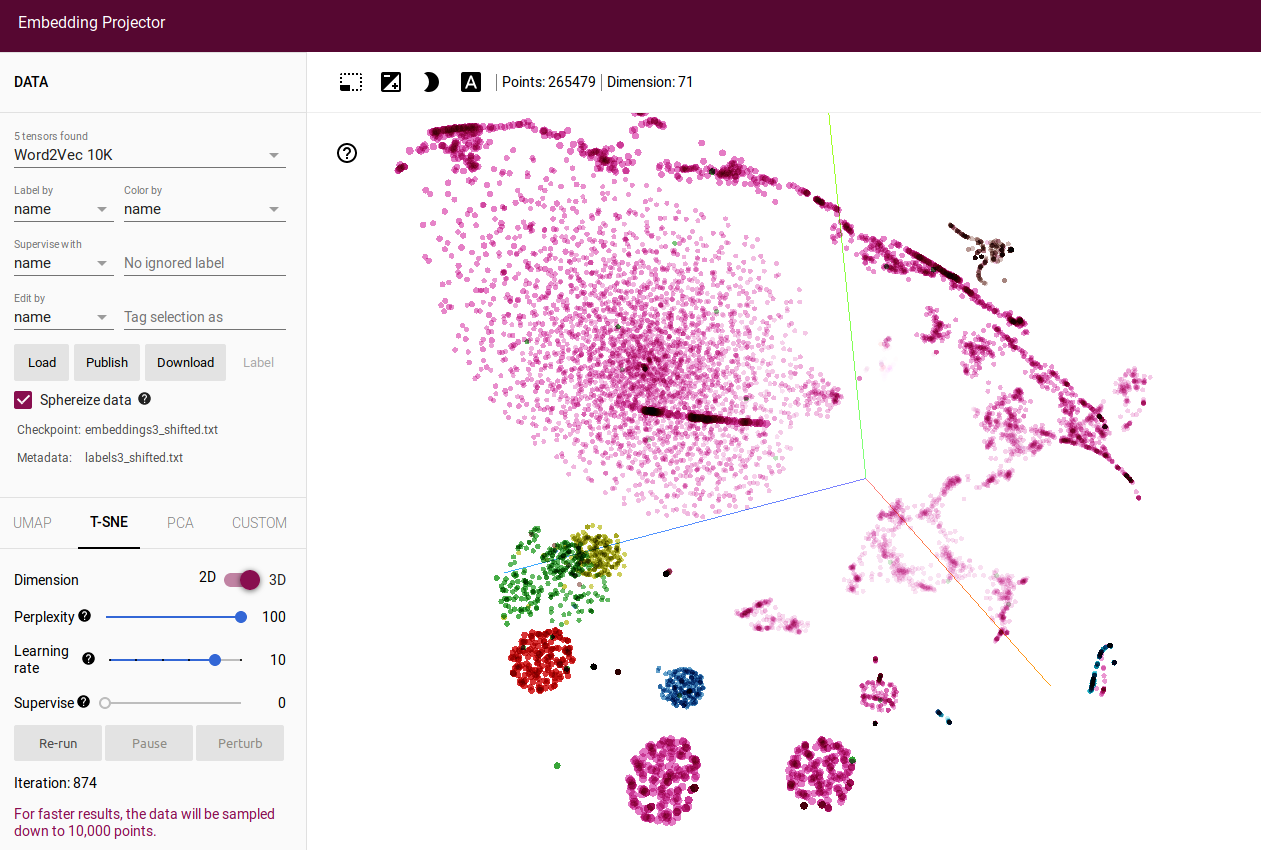
\includegraphics[width=0.8\linewidth]{Figure/dataset3_all_P100_name.png}
	\caption{t-SNE projection of dataset \#3. Color code represents the Yang path that produced each vector.}
	\label{fig:dataset3_all_P100_names}
\end{figure}

Using the \textit{Embedding projector} functionality we are able to isolate the nodes that come from single node, as well as from a specific Yang-path.
We attempt a projection using only the \textbf{leaf1} node, and the \textbf{data-rate} path (the one with most entries), which is shown in figure \ref{fig:dataset3_leaf1_data-rate}.
Although we can see distinction in parts of the data, there are still a big region mixing the two network states of interest.

\begin{figure}[h!]
	\centering
	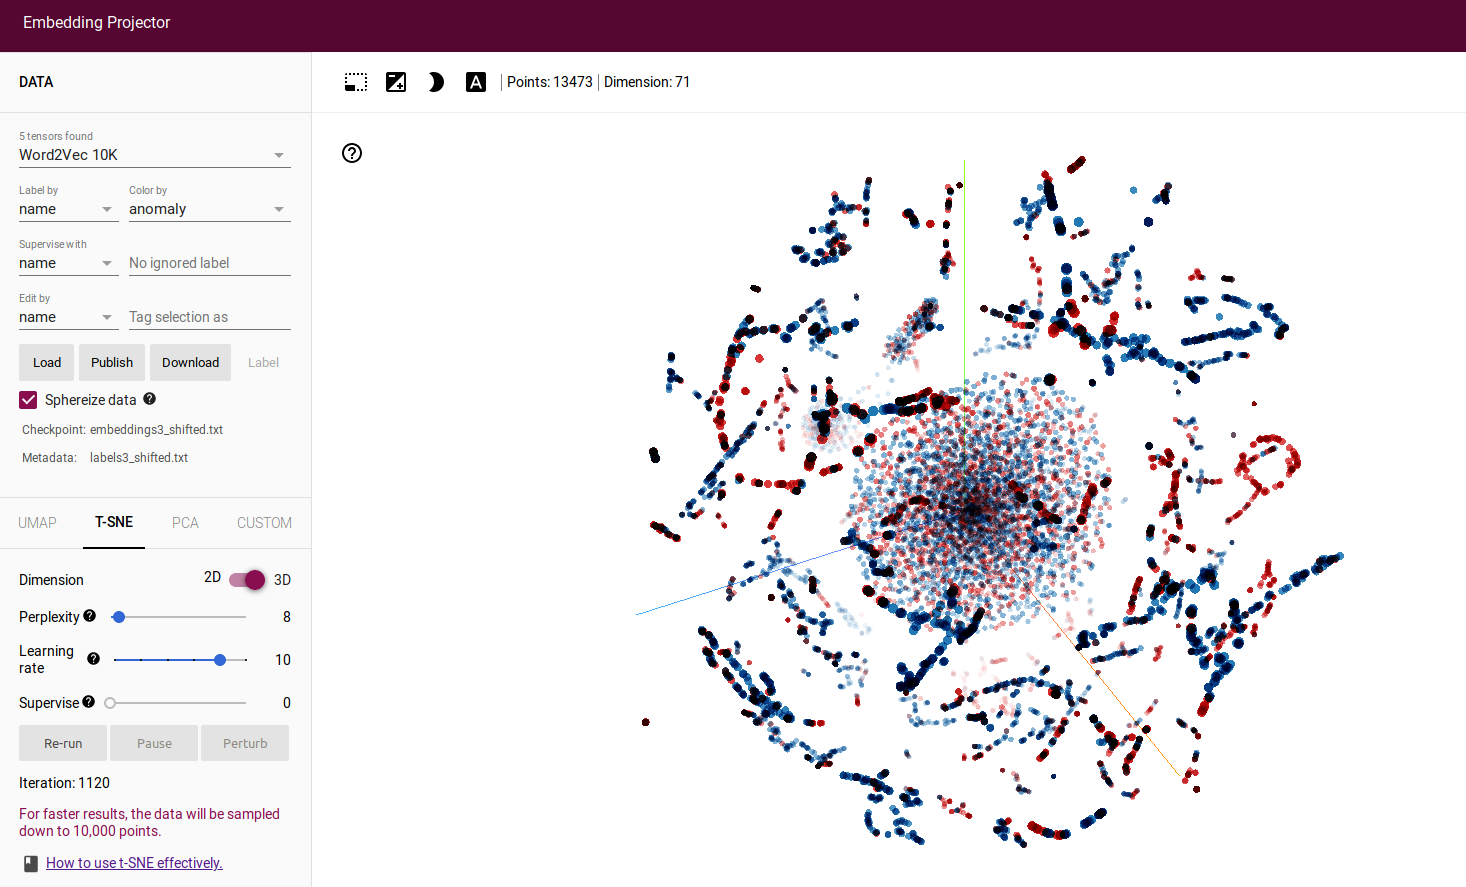
\includegraphics[width=0.8\linewidth]{Figure/dataset3_leaf1_data-rate.png}
	\caption{t-SNE projection of the \textbf{leaf1} node from dataset \#3, using only the features from the \textbf{data-rate} Yang path. The node color distinguish anomalous (red) and normal (blue) states.}
	\label{fig:dataset3_leaf1_data-rate}
\end{figure}

Instead of using pre-selected features, we decide to now project the raw telemetry data available at the \textbf{OutlierDenStream-BigDama18} repository\footnote{https://github.com/anrputina/OutlierDenStream-BigDama18}, which comes separated by node and experiment.
Following Putina et al., we also distinguish between \textit{DataPlane} and \textit{ControlPlane} features to build the node representations for each timestep, discard features which have zero standard deviation, and normalize the resulting data matrix.
Additionaly, the ground truth is used to tag the timesteps where an anomaly is present in the experiment.
The t-SNE projection of node \textbf{leaf1} using the \textit{DataPlane} features is shown in figure \ref{fig:bgpclear_first_leaf1_DP}, where we are able to see a clear distinction between red (anomalous) and blue (normal) network states for this node.

\begin{figure}[h!]
	\centering
	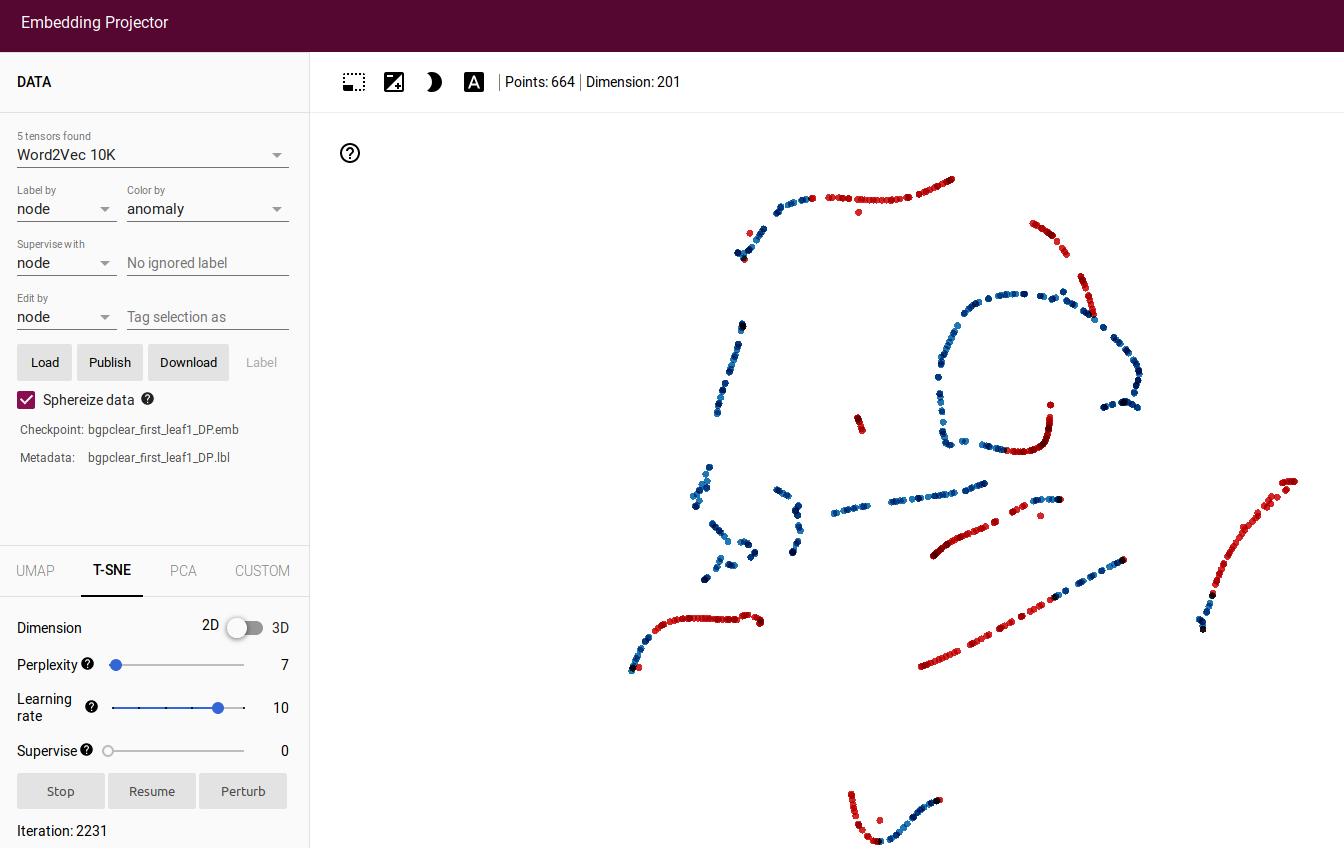
\includegraphics[width=0.8\linewidth]{Figure/bgpclear_first_leaf1_DP.png}
	\caption{t-SNE projection of \textbf{bgpclear\_first}'s \textbf{leaf1} node using \textit{DataPlane} features. Red dots represent timesteps when the system is going through an 'anomaly'}
	\label{fig:bgpclear_first_leaf1_DP}
\end{figure}
\begin{figure}[h!]
	\centering
	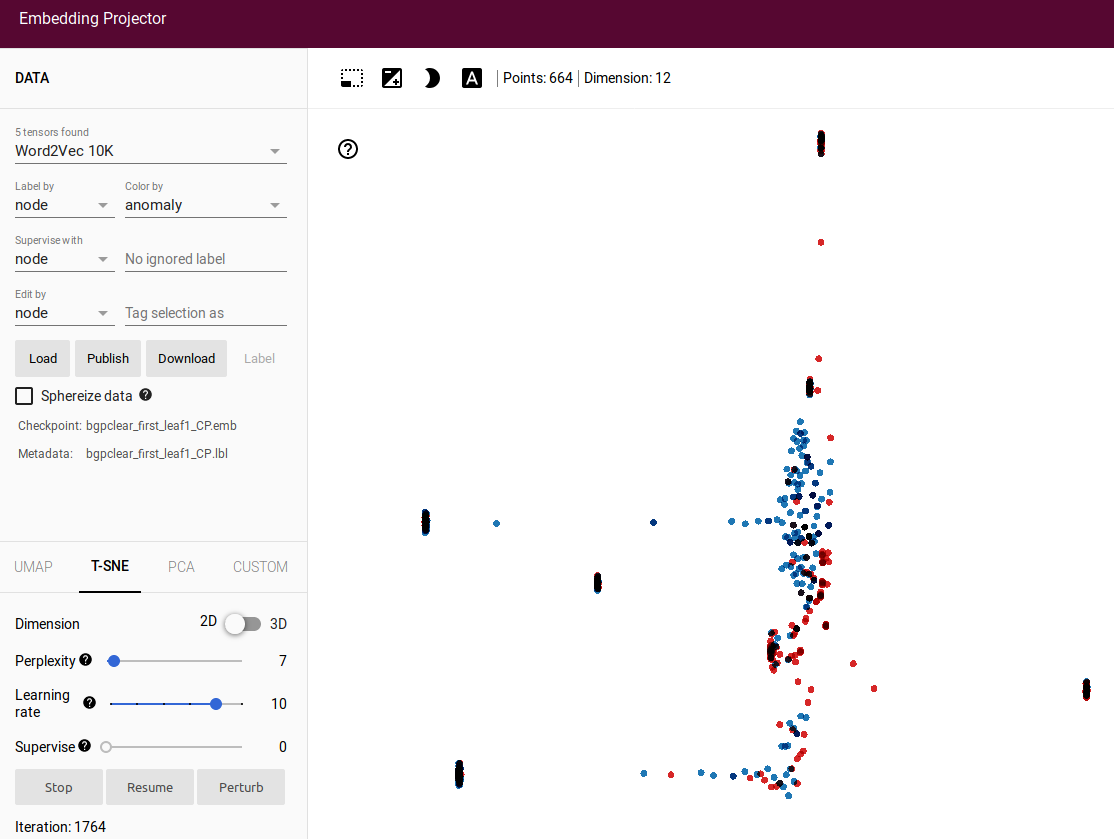
\includegraphics[width=0.8\linewidth]{Figure/bgpclear_first_leaf1_CP.png}
	\caption{t-SNE projection of \textbf{bgpclear\_first}'s \textbf{leaf1} node using \textit{ControlPlane} features. Red dots represent timesteps when the system is going through an 'anomaly'}
	\label{fig:bgpclear_first_leaf1_CP}
\end{figure}

On the other hand, when using the \textit{ControlPlane} for the same node and experiment, we obtain figure \ref{fig:bgpclear_first_leaf1_CP}, which doesn't separate the states of interest as well.

Using data from a different experiment, figure \ref{fig:portflap_first_leaf1_DP} shows that a similar separation of states if found.
\begin{figure}[h!]
	\centering
	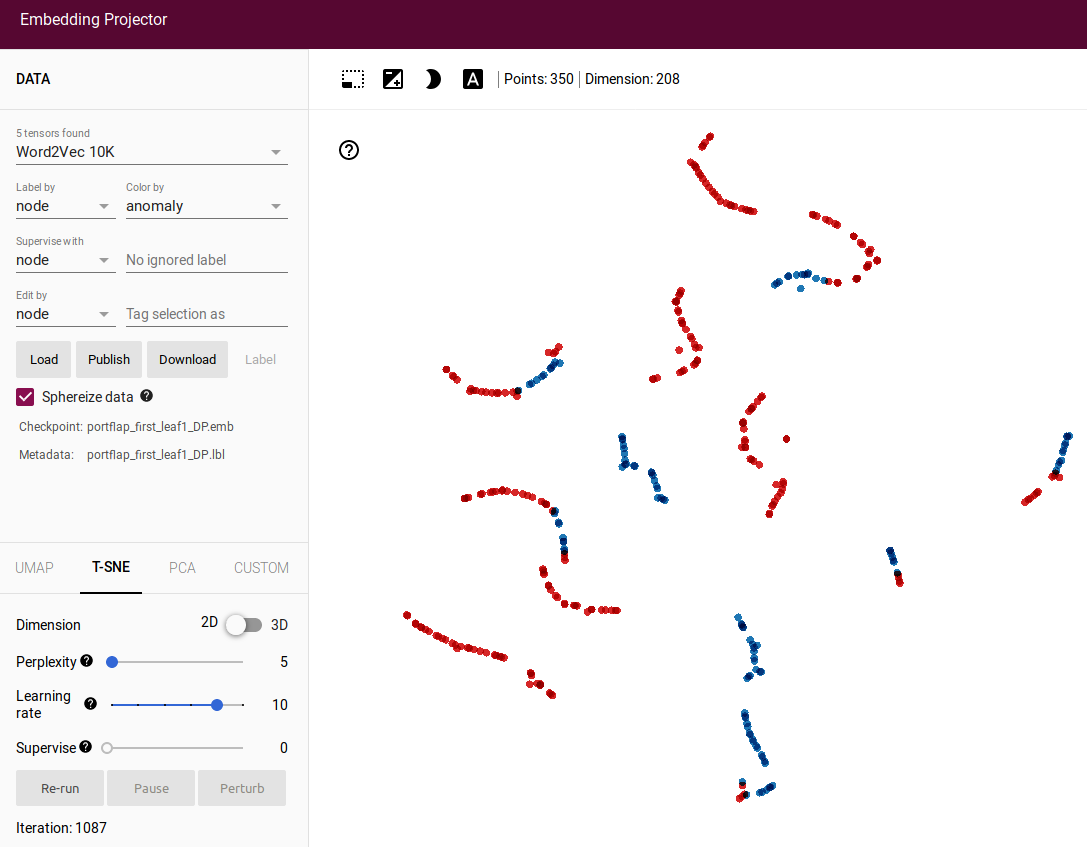
\includegraphics[width=0.8\linewidth]{Figure/portflap_first_leaf1_DP.png}
	\caption{t-SNE projection of \textbf{portflap\_first}'s \textbf{leaf1} node using \textit{DataPlane} features. Red dots represent timesteps when the system is going through an 'anomaly'}
	\label{fig:portflap_first_leaf1_DP}
\end{figure}

This is an interesting result, which shows that it's feasible to subdivide the high-dimensional space in which the given representations exist, and know where the normal behaviour of the network lies.
Additionaly, this can be done without having an expert pre-select the features to use, as done by Putina et al\cite{putina_telemetry-based_2018}.
This subdivision of the space will allow to construct the sequence of tokens that would be processed by the Unsupervised Language Learning pipeline to obtain the network's grammar.





% \newpage
\section{Manufacturing line or multi-machine level}
\label{chapter3}

\textit{Person in Charge; Jin Chenghao and Huang Xinpei}

%---------The scope of this chapter

In this chapter,the researches on energy consumption on the multi-machine/manufacturing line level are introduced.Possible interactions and synergies between different machine tools are considered. Multi-machine ‘ecosystems’ can allow reuse of energy and material flows through proper planning and control.

%---------Define manufacturing line level 

A manufacturing line is a combination of different production processes and typically is composed of diverse machines for processing or transportation as well as personnel. All these production factors are being planned and controlled by a production management system. A multi-machine process boundaries are characterized through Figure \ref{fig:line-boundaries}. 

\begin{figure}[h!]
	\centering
	\includegraphics[width=0.8\linewidth]{Figure/line-boundaries.jpg}
	\caption{System boundaries of a unit process }
	\label{fig:line-boundaries}
\end{figure}

Majority of the energy management literature found in the manufacturing field is at the machine level and focuses on enhancing energy efficiency by selecting optimally either cutting conditions It was discovered that there can be an 80\% reduction in energy consumption if instead of leaving non-bottleneck machines idle, these machines are turned off until needed \cite{Gilles2007}. There have been research efforts that discovered that 85\% of energy in a manufacturing environment is utilized for functions not related to the production of parts \cite{Gutowski2005}. This suggests that with the development of integrated control efforts of system level operations there are many energy savings opportunities for the production line.There has been work into production scheduling that takes into account energy and environmental factors \cite{Fang2011}.There has been a work that proposes a modeling method of task-oriented energy consumption for machining manufacturing system. The energy consumption characteristics driven by task flow in machining manufacturing system are analyzed, which describes that energy consumption dynamically depends on the flexibility and variability of task flow in production processes\cite{He2012}.The Energy Blocks methodology for accurate energy consumption prediction is introduced,which is based on the representation of production operations as segments of specific energy consumption for each operating state of the production equipment and modelling any process chain is possible by arranging the segments according to the production programme\cite{Weinert2011}.There have been some researches on improving energy efficiency in Bernoulli serial lines like Figure \ref{fig:Bernoulli-serial-lines} and a mathematical way of reducing energy cost while maintaining desired production rate is introduced\cite{Wen2016}. 

\begin{figure}[h!]
	\centering
	\includegraphics[width=0.6\linewidth]{Figure/Bernoulli-serial-lines.jpg}
	\caption{Bernoulli serial lines}
	\label{fig:Bernoulli-serial-lines}
\end{figure}

There are also researches that use energy value stream mapping in analyzing the value-added vs. non-value-added energy use in machining cycles\cite{Muller2014}.The foundation for description, acquisition and analysis of all energetic flows into and out of a multi-machine ecosystem are the energy,exergy and entropy concepts.The energy only serves as a carrier of quality,and quality of energy or ’work potential’ can be described by the properties exergy and entropy\cite{Bejan2002}.

\subsection{Process chain design and control}

The energy consumptions are described by the energy to set up the machine and the additional energy used to process the product. That is to say. Energy is divided into two categories: the first one is related to energy required to start up the machine until it reaches ‘ready’ position, which is often fixed for a specific manufacturing process. After setting up a machine, additional requirement is proportional to its processing rate which falls into the second category.Let W$_i$ be the total electrical power consumed,W$_{o_{i}}$ represent the set-up power needed for the machine to reach ‘ready’ status, and k$_{i}p_{i}$ be the additional power, where k$_i$ is a constant, and p$_i$ describes the expected number of parts to be processed per unit of time, which is linearly characterized by the processing rate or capacity of machine i\cite{Wen2016}.

Then we obtain 
\begin{equation} \label{eq:3.1}
\begin{split}
W_{i}=W_{o_{i}}+k_{i}p_{i}
\\
\end{split}
\end{equation}

Then in a serial line with two machines, the system energy consumption within a cycle can be described as:
\begin{equation} \label{eq:3.2}
\begin{split}
E=\sum_{i=1}^{2}W_{o_{i}}+\sum_{i=1}^{2}k_{i}p_{i}
\\
\end{split}
\end{equation}

In such a Bernoulli two-machine line, let PR define the system production rate (i.e. the average number of parts produced by the last machine per unit of time). Then PR can be obtained as follows:
\begin{equation} \label{eq:3.3}
\begin{split}
PR=p_{2}[1-Q(p_{1},p_{2},N)]
\\
\end{split}
\end{equation}

Where,
\begin{equation} \label{eq:3.4}
\begin{split}
Q(p_{1},p_{2},N)=\left\{\begin{matrix}
\frac{(1-p_{1})[1-\alpha(p_{1},p_{2})]}{1-\frac{p_{1}}{p_{2}}\alpha ^{N}(p_{1},p_{2}))} ,if p_{1}\neq p_{2}
\\ 
\frac{1-p_{1}}{N+1-p_{1}}, if p_{1}=p_{2}
\end{matrix}\right.
\\
\end{split}
\end{equation}

\begin{equation} \label{eq:3.5}
\begin{split}
\alpha(p_{1},p_{2})=\frac{p_{1}(1-p_{2})}{p_{2}(1-p_{1})}
\end{split}
\end{equation}

There are two cases considered. One is with constrained workforce, i.e. limited due to capacity shortage or time restriction, while the other addresses the unconstrained case. To start, the constrained case is considered first, i.e. the workforce is limited so that optimal distribution is needed to minimize energy usage and achieve the desired production rate. Introduce workforce constraint p*=p$_1$p$_2$, then the problem is reformulated as follows:
\begin{equation} \label{eq:3.6}
\begin{split}
Min:\sum_{i=1}^{2}W_{o_{i}}+\sum_{i=1}^{2}k_{i}p_{i}
\\
s.t.\left\{\begin{matrix}
PR\geq PR_{d}\\ 
p_{1}p_{2}=p*\\ 
\quad 0<p_{1}<1 \quad 0<p_{2}<1
\end{matrix}\right.
\end{split}
\end{equation}

 Then we can draw a graph of PR-p$_{1}$ in Figure \ref{fig:PR-p1}.
 \begin{figure}[h!]
	\centering
	\includegraphics[width=0.8\linewidth]{Figure/PR-p1.png}
	\caption{PR-p1}
	\label{fig:PR-p1}
\end{figure}
 
 where critical point is P$_1$=$\sqrt{p*}$,p$_{1}'$ and p$_{1}''$ can be obtained by solving the equation:
\begin{equation} \label{eq:3.7}
\begin{split}
p_{1}^{N}(p_{1}-p*)^{N}(PR_{d}p_{1}-p*)+p*^{N+1}(1-p_{1})^{N}(p_{1}-PR_{d})=0 \quad 0<p_{1}<1
\end{split}
\end{equation}
 To minimize energy consumption while satisfying production rate constraint, the author compare the energy critical point with the production rate critical point PR and interval[p1$_{1}'$, p1$_{1}''$].
Researches have been done about the exact analysis for small systems, and the aggregation approach for medium size systems and Heuristic method for large systems\cite{Su2017}.
 
 
\subsection{Local bench marking of manufacturing lines}

Benchmarking is an important step towards forecasting energy use of prospective production lines as well as managing its use in existing lines and setting targets for reducing it. Global benchmarking in energy use can be defined as comparing energy consumption of different equipment at different plants to obtain generic ideal energy use benchmark targets as function of different operating conditions/parameters (i.e. temperature, process plans, schedules, utilization, etc.) as well as equipment characteristics (i.e.age, technology, etc.). Obtaining this extensive information is not always feasible given limited resources, measuring devices, time and information in different plants. Local energy use benchmarking sets local targets within a specific plant or manufacturing system.This has a direct impact on the evaluation of energy use efficiencies and improvement targets in many scenarios where drastic changes to current technology or manufacturing setup are not possible.The overall method of local benchmarking for energy use is composed of six steps in Figure \ref{fig:local-benchmarking}\cite{ElMaraghy2017}.

\begin{figure}[h!]
	\centering
	\includegraphics[width=0.7\linewidth]{Figure/local-benchmarking.jpg}
	\caption{local benchmarking}
	\label{fig:local-benchmarking}
\end{figure}

\subsection{Utilization of energy flows}

Thermoelectric materials are solid-state electrical, and semiconducting properties electricity or electrical power directly with fluid-based systems, such as two-used in smaller-scale applications such electrical-enclosure cooling. More widespread the intrinsic energy-conversion efficiency advancements in system architecture. In a working TE device, segments of p-type- and n-type-doped semiconductor materials, such as suitably doped bismuth telluride, are connected by shunts to form an electric circuit. The shunts are made of an excellent electrical conductor, such as copper. A voltage drives a current through the circuit, passing from one segment to another through the connecting shunts. For determining efficiency, this configuration is equivalent to the electrons passing directly from one TE material to the other. Conventional TE cooling/heating modules are constructed of pairs of TE segments, repeated about 100 times, and organized into ar rays like the one shown in Figure \ref{fig:Thermoelectric materials}\cite{Bell2008}.

\begin{figure}[H]
	\centering
	\includegraphics[width=0.7\linewidth]{Figure/Thermoelectric-materials.png}
	\caption{Thermoelectric materials}
	\label{fig:Thermoelectric materials}
\end{figure}


% \newpage
\section{Factory level}
\subsection{Factory level energy consumption}
\label{chapter 4}

\textit{Person in Charge; Md Sahidul Islam and Wzheng}
%---- the scope of this chapter}}

\subsubsection{Scope}
Energy efficiency has developed into an important objective for industrial enterprises. However, there is still a need for systematic approaches to reduce energy consumption in factories. From an economic point of view, industrial enterprises have an incentive to reduce their energy consumption because of increasing energy prices, such as the European average prices for gas in industry, which rose by approximately 34\% during the last four years \cite{European2013}. 
Despite this situation, the implementation of energy efficiency measures has not met the expectations yet. The reasons for the deficits in realizing energy efficiency include lack of time, lacking transparency on energy consumption, lacking capital for investments and divided responsibilities within a company \cite{Fleiter2013}. 

Product design
Process design
Process adjustments:
Post-processing
plan and implementations


\subsubsection{define factory level}
Different tools and methods have been developed in recent years to support the systematic analysis and optimization of industrial enterprises for reducing their energy consumption. However, the existing methods mainly focus on product design, Process design, process adjustment, manufacturing processes, machine process and smart factory building design. Although these are important aspects of the energy-efficient factory, considering the interrelationships between products, processes and resources in the factory system is essential for a holistic integration of energy efficiency in the enterprise. 

\subsubsection{factory building energy consumption }
The starting point for the approach is the definition of the project task or planning situation by the factory planning participant (user input). The most important parameters to describe the task are object level, system process, part of the energy chain, energy form, planning case and user’s role. According to their background, the first four parameters are defined as technical parameters and the last two as organizational parameters. 

The object level describes the level of abstraction of the considered system (e.g. factory, building, plant area, single machine). The system process defines the process of the enterprise to which the considered system belongs to (e.g. assembly, logistics). The part of the energy chain describes whether the system performs energy generation, conversion, distribution, storage or use, since factories increasingly integrate several of these functions \cite{Muller2013a}. The energy form defines the types of resources that are used within the considered system (e.g. electricity, water). The planning case comprises the extent to which changes are possible in the system; planning a new system has the highest degrees of freedom, whereas operating the existing system equals the lowest degree of freedom. Finally, the user's role defines the perspective of the user (e.g. factory planner, worker). 

the implementing methods is the high effort for data acquisition. Therefore, an approach to reduce energy consumption within factory systems was developed that provides energy efficiency measures to factory planning participants based on qualitative data \cite{Muller2013}.

Herrmann et al.\cite{Herrmann2011} proposed a holistic definition of factory management, including technical building services as an important player \cite{Herrmann2011}. Seow and Rahimifard outlined a framework for modelling energy consumption within a manufacturing system from a product’s viewpoint, and utilized the energy data at factory and process levels \cite{Seow2011}. Mouzon et al. proposed a mathematics programming model to optimize the total energy consumption of manufacturing \cite{Gilles2007}. Clearly, a comprehensive energy consumption models at this level is still lacking. 

Manuela Krones and Egon Müller \cite{Krones2014} developed a general concept has been developed to systematically guide a factory planning participant from his or her project task to appropriate energy efficiency measures. We introduce their work in detail here. The goal is to provide suitable energy efficiency approaches in order to increase the efficiency of information gathering. The approach consists of four major steps, which are explained in the following.


When applying the method, not all of these parameters need to be specified. The user can choose which parameters to specify; however, if the number of specified parameters is too small, the user may receive too unspecific results and needs to repeat the approach with changes in the input. 

\begin{figure}[h!]
	\centering
	\includegraphics[width=0.6\linewidth]{Figure/Overall-concept-methods.jpg}
	\caption{Overall concept for methodical approach to systematically identify energy efficiency measures}
	\label{fig:overalconcept}
\end{figure}


\subsection{Smart Factory Building}
Firstly did research on the relation between green buildings, smart buildings, and energy efficiency. To realize how they relate each other together with energy usage, and consequently putting deeper attention on the factors that have a direct impact on consumption. We also generated an economic model based on information concerning: energy consumption and distribution in different types of buildings, prices of energy, average savings due to the implementation of smart technologies, and prices of smart technologies. 
Here we will mention some interesting energy efficiency measures that are strictly related to the energy consumption in buildings and that would be close to composing all the aspects related with that in a project like this. As figure shows a general classification of the influencing systems.

\begin{figure}[h!]
	\centering
	\includegraphics[width=0.8\linewidth]{Figure/FacturyEnergyConcumption.png}
	\caption{Smart factory building design conceptual approach}
	\label{fig:factoryenergyconsumption}
\end{figure}


\subsection{Heating, ventilation, and air conditioning (HVAC)}

\subsubsection{Heating }
Heaters are appliances whose purpose is to generate heat (i.e. warmth) for the building. This can be done via central heating. Such a system contains a boiler, furnace, or heat pump to heat water, steam, or air in a central location such as a furnace room in a home, or a mechanical room in a large building. The heat can be transferred by convection, conduction, or radiation. Since the new AHU system has heat recovery, this section takes into account that 80% of the supply air is already heated exhaust air. 

\subsubsection{Ventilation }
Ventilation is the process of changing or replacing air in any space to control temperature or remove any combination of moisture, odors, smoke, heat, dust, airborne bacteria, or carbon dioxide, and to replenish oxygen. Ventilation includes both the exchange of air with the outside as well as circulation of air within the building. It is one of the most important factors for maintaining acceptable indoor air quality in buildings. Methods for ventilating a building may be divided into mechanical/forced and natural types.The energy consumption in a single air handling unit, or process, can be noticed in the
enthalpy’s change over time.

\subsubsection{Air Conditioning }
An air conditioning system, or a standalone air conditioner, provides cooling and humidity control for all or part of a building. Air conditioned buildings often have sealed windows, because open windows would work against the system intended to maintain constant indoor air conditions. Outside, fresh air is generally drawn into the system by a vent into the indoor heat exchanger section, creating positive air pressure. The percentage of return air made up of fresh air can usually be manipulated by adjusting the opening of this vent. Typical fresh air intake is about 10%.

\subsubsection{Cooling}
cooling systems can have very high efficiencies, and are sometimes combined with seasonal thermal energy storage so that the cold of winter can be used for summer air conditioning. Common storage mediums are deep aquifers or a natural underground rock mass accessed via a cluster of small-diameter, heat-exchanger-equipped boreholes. Some systems with small storage's are hybrids, using free cooling early in the cooling season, and later employing a heat pump to chill the circulation coming from the storage. The heat pump is added-in because the storage acts as a heat sink when the system is in cooling (as opposed to charging) mode, causing the temperature to gradually increase during the cooling season.

recovery: The use of heat/enthalpy wheels and energy recovery ventilator allow them to absorb moisture from the air while at the same time cooling the air that is absorbed, to finally exhaust heated air. It is a system that allows the capacity of the HVAC system to be reduced since it can be used in both summer andwinter months. In summer it would take the heat and humidity outside the building while in winter it would exhaust the recovered heat inside the building (2015). Infrared heaters: These alternative devices can be powered electrically, by propane or with natural gas. The increase in efficiency is due to the higher impassivity the can produce compared with traditional heaters, even if in most of the cases their combustion efficiency is lower. Solar systems: Using the sun to heat water and use this thermal storage to heat the building is both cost and energy efficient. Cooling systems: When talking about this, we have to also mention the refrigeration systems. And there are three things when considering efficiency in these systems: energy usage, type and quantity of heat exhausted and refrigerant type. The air-cooled systems are the most spread used and as in many cases, the traditional equipment is not optimal in terms of energy efficiency (2017).

\begin{table}[H]
\centering
\caption{Definition of symbols \cite{Watson2018}}
\label{table:symbols}
\begin{tabular}{llll}
\hline
& 2020 & 2030 & 2050 \\ \hline
Greenhouse gas reduction & 20\% & 40\%  & 80\% \\
Energy production from renewable & 20\% & 27\% & \\
Energy efficiency improvement & 20\% & 27\% & \\ \hline
\end{tabular}

\end{table}

Energy efficiency improvement Emissions reductions in the last years have been reduced mainly thanks to progress on renewable and on energy efficiency measures. However, from the three targets of the European Union, the only one that will not be achieved by 2020 will be the one regarding improvement in energy efficiency (European Commission, 2017 \cite{European2013}). It is due to a number of barriers that go out of the scope of this project, but in general, they are related with financial uncertainty, cultural behaviors and lack of knowledge on energy efficiency measures.

We need to investigate towards several directions in order to make factories more energy efficient. General issues to be solved include:

\begin{itemize}  
\item An inter operable infrastructure that allows us to on-line monitor energy consumption down to discrete device level
\item Concrete models for energy consumption prediction at each layer e.g. device level, location, process level etc
\item Enterprise services that evaluate and assist in optimizing plans and processes dynamically based on their energy usage e.g. at production, at supply chain, etc
\item Applicability of Market driven mechanisms and close collaboration with energy providers for optimal energy usage / Integration of the distributed alternative energy resources
\item Support for software management for large scale infrastructures e.g. remote monitoring, remote diagnostics,
\end{itemize}

The application when a technician is accessing the main view of the building. Here the five different administrative domains can be accessed by pressing on the desired floor. Moreover, important events are listed on the left part of the window and the user can click on them to directly access the device emitting the alert.

\subsection{<>Conclusion }
When exceeding the level of milt machine chains, simulation techniques become predominant to master the complexity of predicting energy and resource flows for larger manufacturing systems.
Technical building services can consume considerable amounts of energy:
It is obvious that factory layout and facility optimization need careful attention in a design stage.
Just like residential buildings, production facilities need to be constructed according to state of the art building physics principles, thus minimizing energy inputs for HVAC   conditioning of the work environment, while taking into account local climate conditions.
Similar to the multi-machine strategy, production planning can be optimized at a facility wide level in order to limit the total energy consumption.




% \newpage
\section{Summary}


This article includes the study on energy consumption on multiple levels; the first part of the work shows the importance of energy consumption in manufacturing industry. The research find that the big amount of energy consumed during manufacturing and the importance of energy savings. The study about the macroscopic view for the industry energy cost showed the importance of studying energy consumption and efficient improvement. 

The outline of the 
graph showed the energy consumption, literature review for energy consumption in manufacturing industry from machine to factory level. For machine level, a general method is shown for the calculation of energy consumption. An inventory of different machining processes are made and are based on the overall life cycle analysis. The possible improvement strategies are provided for a general process and for four specific processes. After that, the energy analyze for multi-machine system shows the energy connection of machines, together with the energy flows simulation. At last, review of factory level energy consumption is conducted, and investigate towards several directions in order to make factories more energy efficient for further discussion. 

Analysis of energy consumption is a major part in understanding a machine, factory. A combination of models, software and measurements is necessary to perform such an analysis. When done correctly, bottleneck machines can be discovered for manufacturing line levels or high energy consumption sub-process are brought to light in machine level. Energy improvement is done from the start of building or choosing machine/manufacturing line until the end when it is dismantled. Improvement strategies are similar over all the levels, e.g. energy management, new components or machines, etc.

An integrated effort over all the levels is necessary when we want to see a big improvement in energy consumption. Duflou et al. \cite{Duflou2012} predicts a 50\% improvement when global improvements are made in manufacturing

This study reviewed, a wide variety of considerations with relation to environmental impact reducing measures in general and energy and resource efficiency in specific has been discussed and the identified methods and techniques for analysis and system optimization.







\newpage
%bibliography
\bibliographystyle{abbrv}
\bibliography{CAiN.bib}

\end{document}